\begin{frame}{Introdução}
    \begin{block}{Qual o problema a ser abordado?}
        \begin{itemize}
            \item realizar a caracterização hidrológica e modelagem Chuva-Vazão
            \item prever enchentes pelo HEC-HMS e por aprendizado profundo (minha parte)
            \item principais bacias hidrográficas de Minas Gerais
            \item Bacias:
            \begin{itemize}
               \item rio São Francisco
               \item rio Doce
               \item rio Jequitinhonha
               \item rio Paraíba do Sul
               \item rio Grande
            \end{itemize}
        \end{itemize}
    \end{block}
\end{frame}

\begin{frame}{Introdução}
    \begin{figure}
        \centering
        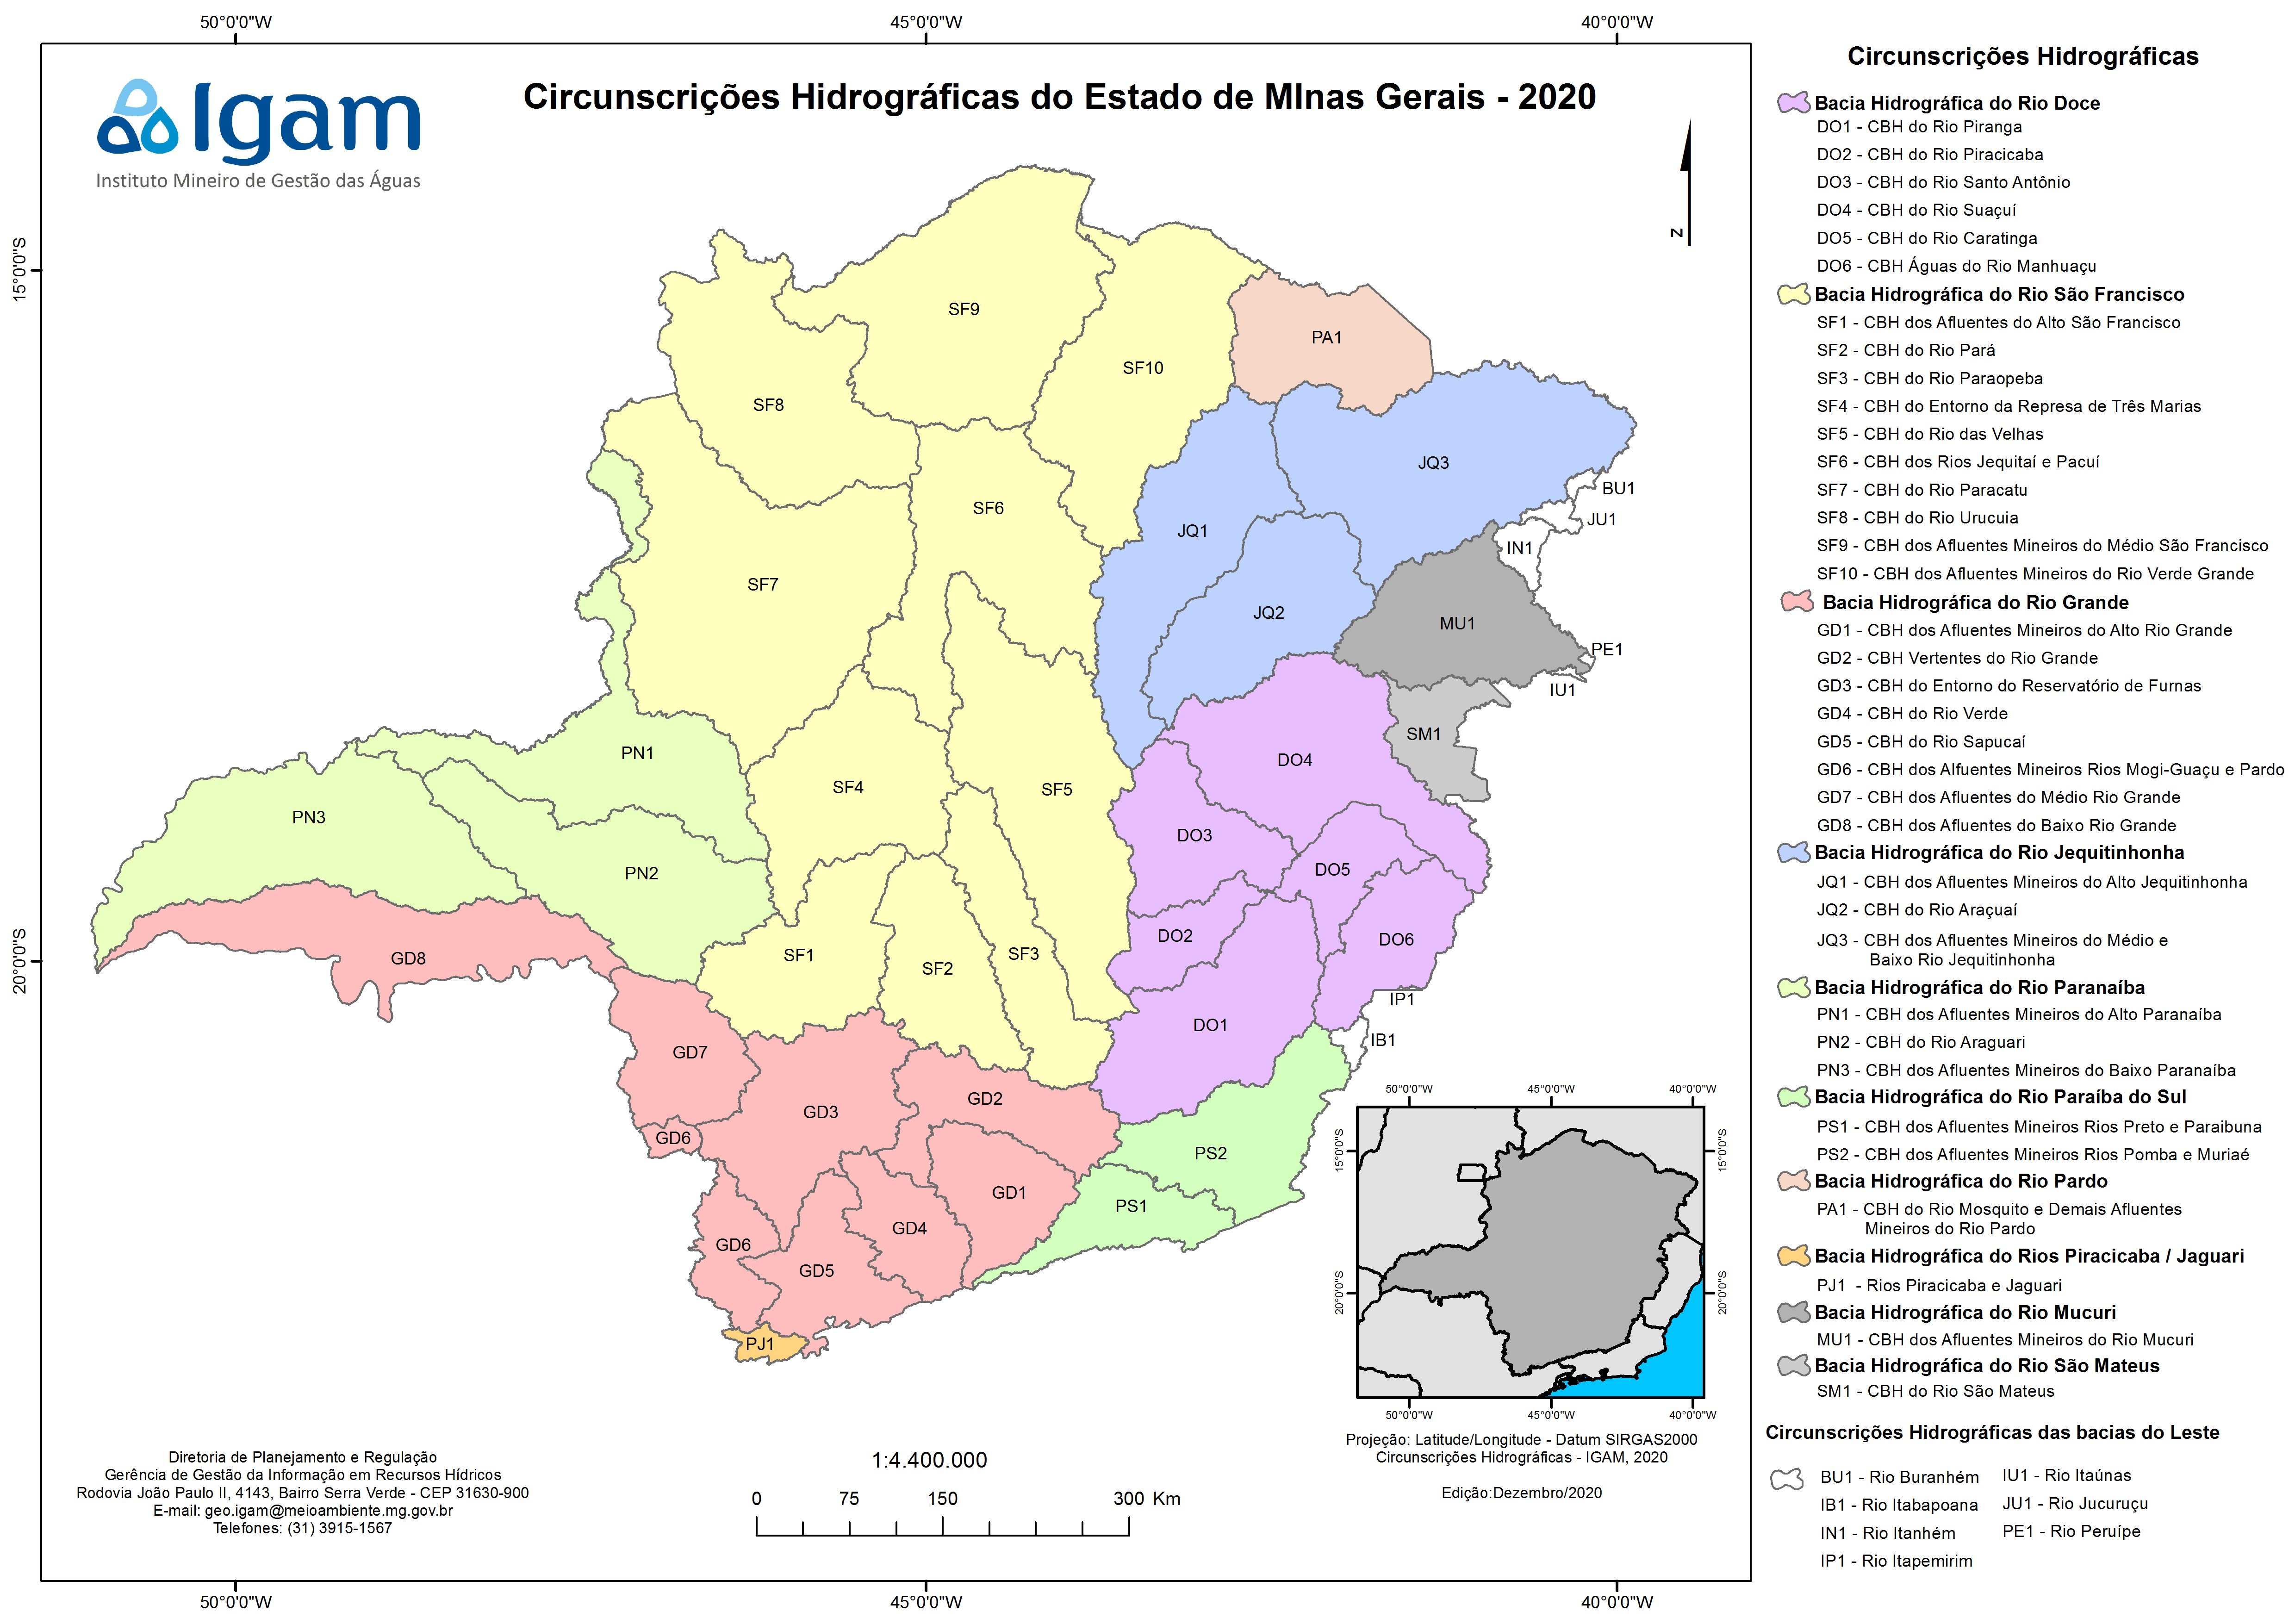
\includegraphics[width=10cm]{img/bacias.png} \\
        Fonte: Inst. Mineiro de Gestão das Águas - IGAM
        \label{fig:bacias}
    \end{figure}
\end{frame}
